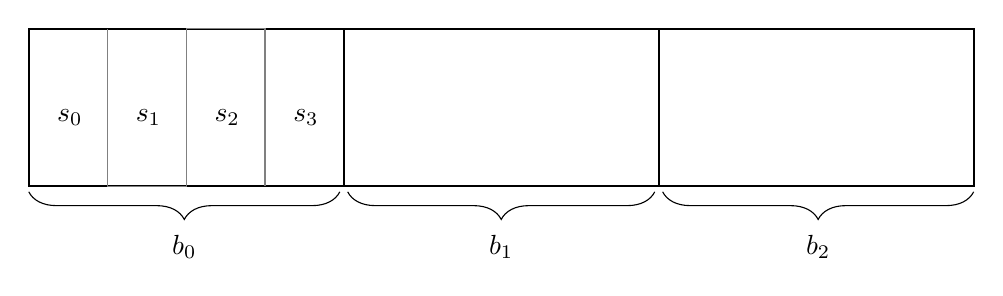
\begin{tikzpicture}
  \draw[thick](0,2,2)--(12,2,2)--(12,0,2)--(0,0,2)--(0,2,2)--(8,2,2)--(8,0,2)--(4,0,2)--(4,2,2);
  \draw[gray](1,2,2)--(1,0,2)--(2,0,2)--(2,2,2)--(3,2,2)--(3,0,2);
  \node at (-0.25,0.1,0) {$s_0$}; 
  \node at (0.75,0.1,0) {$s_1$}; 
  \node at (1.75,0.1,0) {$s_2$}; 
  \node at (2.75,0.1,0) {$s_3$}; 

\draw [decorate,decoration={brace,amplitude=10pt, mirror},xshift=0pt,yshift=-2pt]
(0,0,2) -- (3.95,0,2)node [black,midway,yshift=-20pt] {$b_0$};
\draw [decorate,decoration={brace,amplitude=10pt, mirror},xshift=0pt,yshift=-2pt]
(4.05,0,2) -- (7.95,0,2)node [black,midway,yshift=-20pt] {$b_1$};
\draw [decorate,decoration={brace,amplitude=10pt, mirror},xshift=0pt,yshift=-2pt]
(8.05,0,2) -- (12,0,2)node [black,midway,yshift=-20pt] {$b_2$};
  
\end{tikzpicture}